\begin{name}
	{Biên soạn: Thầy Toan Vo, Thầy Đỗ Đường Hiếu \& Phản biện: Thầy Đỗ Đường Hiếu, Thầy Toan Vo}
	{Đề thi giữa học kỳ 1 năm học 2020-2021, THPT Hiệp Đức, Quảng Nam}
\end{name}
\setcounter{ex}{0}\setcounter{bt}{0}
\Opensolutionfile{ans}[ans/ans-2-GHK1-28-HiepDuc-QuangNam-21]
\begin{ex}%[Giữa học kỳ I, THPT Hiệp Đức, Quảng Nam, 2021]%[Toan Vo, 12EX3-2021]%[2D1B1-2]
Cho hàm số $y=f(x)$ có bảng biến thiên như hình vẽ sau.
\begin{center}

\begin{tikzpicture}[>=stealth]
	\tkzTabInit[nocadre=false,lgt=1.5,espcl=2,deltacl=0.5]{$x$/.6 ,$f'(x)$/.6,$f(x)$/2}
	{$-\infty$, $-3$, $0$ , $3$ , $+\infty$}
	\tkzTabLine{, -,$0$,+,$0$ , - , $0$ , + , }
	\tkzTabVar{+/$+\infty$, -/$-1$, +/$1$ , -/$-1$ , +/$+\infty$}
\end{tikzpicture}
\end{center}
Hàm số đã cho đồng biến trên khoảng nào dưới đây?
\choice
{\True $(-3;0)$}
{$(-3;3)$}
{$(0;3)$}
{$(-\infty;-3)$}
\loigiai
{
Từ bảng biến thiên, hàm số $y=f(x)$ đồng biến trên khoảng $(-3;0)$ và $(3;+\infty)$.
}
\end{ex}
\begin{ex}%[Giữa học kỳ I, THPT Hiệp Đức, Quảng Nam, 2021]%[Toan Vo, 12EX3-2021]]%[2D1B1-2]
Cho hàm số $y=f(x)$ có bảng xét dấu đạo hàm như sau.
\begin{center}

\begin{tikzpicture}[>=stealth]
	\tkzTabInit[nocadre=false,lgt=1.5,espcl=2,deltacl=0.5]{$x$/.6 ,$y'$/.6}
	{$-\infty$, $-2$, $0$ , $2$ , $+\infty$}
	\tkzTabLine{,+,$0$,-,d,-,$0$,+,}
\end{tikzpicture}
\end{center}
Mệnh đề nào dưới đây đúng?
\choice
{\True Hàm số đồng biến trên khoảng $(2;3)$}
{Hàm số nghịch biến trên khoảng $(-2;2)$}
{Hàm số nghịch biến trên khoảng $(-\infty;-2)$}
{Hàm số đồng biến trên khoảng $(-\infty;0)$}
\loigiai
{
Ta thấy $y'>0$ trên khoảng $(2;3)$ nên hàm số $y=f(x)$ đồng biến trên khoảng $(2;3)$.
}
\end{ex}
\begin{ex}%[Giữa học kỳ I, THPT Hiệp Đức, Quảng Nam, 2021]%[Toan Vo, 12EX3-2021]%[2D1Y1-1]
Hàm số nào dưới đây đồng biến trên $\mathbb{R}$?
\choice
{\True $y=3x^3+3x-2$}
{$y=x^4+3x^2$}
{$y=2x^3-5x+1$}
{$y=\dfrac{x-2}{x+1}$}
\loigiai
{
Xét hàm số $y=3x^3+3x-2$, ta có $y'=9x^2+3>0$, $\forall x\in\mathbb{R}$. Nên hàm số $y=3x^3+3x-2$ đồng biến trên $\mathbb{R}$.
}
\end{ex}
\begin{ex}%[Giữa học kỳ I, THPT Hiệp Đức, Quảng Nam, 2021]%[Toan Vo, 12EX3-2021]%[2D1B1-3]
Tìm số các giá trị nguyên của tham số $m$ trong đoạn $[-10;10]$ để hàm số $y=mx^3+mx^2+(m+1)x-3$ nghịch biến trên $\mathbb{R}$.
\choice
{\True $9$}
{$21$}
{$10$}
{$8$}
\loigiai
{
Ta có $y'=3mx^2+2mx+m+1$. Để $y'\le0$, $\forall x\in\mathbb{R}$ thì
\[\heva{&3m<0\\&\Delta'=m^2-3m^2-3m\le0}\Leftrightarrow\heva{&m<0\\&2m^2+3m\ge0}\Leftrightarrow\hoac{&m<0\\&m\ge0\vee m\le -\dfrac{3}{2}}\Leftrightarrow m\le-\dfrac{3}{2}.\]
Do $m\in\mathbb{Z}$ và $m\in[-10;10]$ nên $m\in\{-2;-3;-4;-5;-6;-7;-8;-9;-10\}$.\\
Do đó có $9$ giá trị nguyên của $m$ thỏa mãn yêu cầu bài toán.
}
\end{ex}
\begin{ex}%[Giữa học kỳ I, THPT Hiệp Đức, Quảng Nam, 2021]%[Toan Vo, 12EX3-2021]%[2D1B2-2]
Cho hàm số $y=f(x)$ có bảng biến thiên như hình vẽ sau.
\begin{center}

\begin{tikzpicture}[>=stealth]
	\tkzTabInit[nocadre=false,lgt=1.5,espcl=2,deltacl=0.5]{$x$/.6 ,$f'(x)$/.6,$f(x)$/2}
	{$-\infty$, $0$ , $3$ , $+\infty$}
	\tkzTabLine{,+,$0$ , - , $0$ , + , }
	\tkzTabVar{-/$-\infty$, +/$2$ , -/$-4$ , +/$+\infty$}
\end{tikzpicture}
\end{center}
Hàm số đã cho đạt cực tiểu tại điểm nào?
\choice
{\True $x=3$}
{$x=0$}
{$x=2$}
{$x=-4$}
\loigiai
{
Từ bảng biến thiên, hàm số đã cho đạt cực tiểu tại điểm $x=3$ với $y=-4$.
}
\end{ex}
\begin{ex}%[Giữa học kỳ I, THPT Hiệp Đức, Quảng Nam, 2021]%[Toan Vo, 12EX3-2021]%[2D1B2-2]
Cho hàm số $f(x)$ liên tục trên $\mathbb{R}$ và có bảng xét dấu của $f'(x)$ như sau.
\begin{center}

\begin{tikzpicture}[>=stealth]
	\tkzTabInit[nocadre=false,lgt=1.5,espcl=2,deltacl=0.5]{$x$/.6 ,$f'(x)$/.6}
	{$-\infty$, $-2$, $1$ , $2$ , $3$, $+\infty$}
	\tkzTabLine{,-,$0$,+,$0$,-,d,+,$0$,+,}
\end{tikzpicture}
\end{center}
Tìm số điểm cực tiểu của hàm số đã cho.
\choice
{\True $2$}
{$4$}
{$3$}
{$1$}
\loigiai
{
Ta có $f'(x)$ đổi dấu từ âm sang dương qua hai điểm $x=-2$ và $x=2$.\\
Do $f(x)$ liên tục nên hàm số $y=f(x)$ có hai điểm cực tiểu là $x=-2$ và $x=2$.
}
\end{ex}
\begin{ex}%[Giữa học kỳ I, THPT Hiệp Đức, Quảng Nam, 2021]%[Toan Vo, 12EX3-2021]%[2D1B2-1] 
Tìm điểm cực tiểu của đồ thị hàm số $y=-x^3+3x+1$.
\choice
{\True $M(-1;-1)$}
{$Q(1;3)$}
{$N(0;1)$}
{$P(2;-1)$}
\loigiai
{
Ta có $y'=-3x^2+3$ và $y''=-6x$. Để $x=x_0$ là điểm cực tiểu của hàm số thì
\[\heva{&y'(x_0)=0\\&y''(x_0)>0}\Leftrightarrow\heva{&-3x_0^2+3=0\\&-6x_0>0}\Leftrightarrow\heva{&x_0=1\vee x_0=-1\\&x_0<0}\Leftrightarrow x_0=-1.\]
Khi đó $y(x_0)=-(-1)^3+3(-1)+1=-1$.\\
Do đó điểm $M(-1;-1)$ là điểm cực tiểu của đồ thị hàm số $y=-x^3+3x+1$.
}
\end{ex}
\begin{ex}%[Giữa học kỳ I, THPT Hiệp Đức, Quảng Nam, 2021]%[Toan Vo, 12EX3-2021]%[2D1B2-3]
Tìm tập hợp tất cả các giá trị thực của tham số $m$ để hàm số $y=x^3+(3m-1)x^2+m^2x-3$ đạt cực tiểu tại $x=-1$.
\choice
{\True $\{5\}$}
{$\{5;1\}$}
{$\{1\}$}
{$\varnothing$}
\loigiai
{
Ta có $y'=3x^2+(6m-2)x+m^2$ và $y''=6x+6m-2$.\\
Với $m=0$ thì hàm số trở thànH $y=-3$, không đồng biến hay nghịch biến.\\
Để hàm số đạt cực tiểu tại $x=-1$ thì
\[\heva{&y'(-1)=0\\&y''(-1)>0}\Leftrightarrow\heva{&3-6m+2+m^2=0\\&-6+6m-2>0}\Leftrightarrow\heva{&m=1\vee m=5\\&m>\dfrac{4}{3}}\Leftrightarrow m=5.\]
Vậy $m=5$ thỏa mãn yêu cầu bài toán.
}
\end{ex}
\begin{ex}%[Giữa học kỳ I, THPT Hiệp Đức, Quảng Nam, 2021]%[Toan Vo, 12EX3-2021]%[2D1G2-6]
Tìm tất cả các giá trị của tham số thực $m$ để đường thẳng đi qua hai điểm cực trị của đồ thị hàm số $y=x^3-3mx+2$ cắt đường tròn $(C)$ có tâm $I(1;1)$, bán kính bằng $1$ tại hai điểm phân biệt $A$, $B$ sao cho diện tích tam giác $IAB$ đạt giá trị lớn nhất.
\choice
{\True $m=\dfrac{2\pm\sqrt{3}}{2}$}
{$m=\dfrac{2\pm\sqrt{3}}{3}$}
{$m=\dfrac{1\pm\sqrt{3}}{2}$}
{$m=\dfrac{2\pm\sqrt{5}}{2}$}
\loigiai
{
Ta có $y'=3x^2-3m$. Biến đổi $y=\dfrac{x}{3}(3x^2-3m)-2mx+2$.\\
Gọi $C(x_C;y_C)$ và $D(x_D;y_D)$ là hai điểm cực trị của đồ thị hàm số.\\
Khi đó $y'(x_C)=y'(x_D)=0$, suy ra $y_C=-2mx_C+2$ và $y_D=-2mx_D+2$.\\
Do đó đường thẳng đi qua hai điểm cực trị $C$ và $D$ có phương trình $(\Delta) \colon y=-2mx+2$.\\
Đường tròn $(C)$ có tâm $I(1;1)$ và bán kính $R=1$ nên có phương trình $(C)\colon (x-1)^2+(y-1)^2=1$.\\
$\Delta$ cắt $(C)$ tại hai điểm $A$, $B$ nên $\triangle IAB$ cân tại $I$ và có diện tích là
$$S=\dfrac{1}{2} \cdot IA \cdot IB \cdot \sin \widehat{AIB}= \dfrac{1}{2} \cdot \sin \widehat{AIB}.$$
Diện tích $S$ lớn nhất khi $\sin \widehat{AIB}=1 \Leftrightarrow \widehat{AIB}=90^\circ$.\\
Ta có $\triangle IAB$ vuông cân tai $I$ và $IA=IB=1$.\\
Nên khoảng cách từ $I$ đến $\Delta \colon 2mx+y-2=0$ là $d(I; \Delta)= \dfrac{1}{2} AB = \dfrac{1}{2} \sqrt{2} =\dfrac{\sqrt{2}}{2}$. Suy ra 
  \begin{eqnarray*}
  && d(I; \Delta)=\dfrac{\sqrt{2}}{2}\\
  & \Leftrightarrow & \dfrac{|2m-1|}{\sqrt{4m^2+1}}=\dfrac{\sqrt{2}}{2}\\
   & \Leftrightarrow & 2|2m-1|=\sqrt{8m^2+2}\\
    & \Leftrightarrow & 4(4m^2-4m+1)=8m^2+2\\
      & \Leftrightarrow & 8m^2-16m+2=0\\
      & \Leftrightarrow & m=\dfrac{2\pm\sqrt{3}}{2}.
  \end{eqnarray*}
}
\end{ex}
\begin{ex}%[Giữa học kỳ I, THPT Hiệp Đức, Quảng Nam, 2021]%[Toan Vo, 12EX3-2021]%[2D1Y3-1]
Cho hàm số $y=f(x)$ liên tục trên $[-3;2]$ và có bảng biến thiên như sau
\begin{center}

\begin{tikzpicture}[>=stealth]
	\tkzTabInit[nocadre=false,lgt=1.5,espcl=2,deltacl=0.5]{$x$/.6 ,$f'(x)$/2}
	{$-3$, $-1$, $0$ , $1$ , $2$}

	\tkzTabVar{-/$-2$, +/$3$, -/$1$ , +/$2$ , -/$0$}
\end{tikzpicture}
\end{center}
Gọi $M, m$ lần lượt là giá trị lớn nhất và giá trị nhỏ nhất của hàm số $y=f(x)$ trên đoạn $[-1;2] $. Tính $M+m $.
\choice
{$1$}
{$2$}
{\True $3$}
{$4$}
\loigiai
{
Trên đoạn $[-1;2] $ hàm số có $M=3$ và $m=0$ nên $M+m=3$.
}
\end{ex}
\begin{ex}%[Giữa học kỳ I, THPT Hiệp Đức, Quảng Nam, 2021]%[Toan Vo, 12EX3-2021]%[2D1Y3-1]
Tìm giá trị lớn nhất $M$ của hàm số $y=\dfrac{3 x-1}{x-3}$ trên đoạn $[0 ; 2]$.
\choice
{$M=\dfrac{1}{3}$}
{$M=-\dfrac{1}{3}$}
{$M=-5$}
{$M=5$}
\loigiai
{
Trên đoạn  $[0 ; 2]$ ta có $y'=\dfrac{-8}{(x-3)^2} <0$ nên hàm số nghịch biến.\\
Hơn nữa, $y(0)=\dfrac{1}{3},\, y(2)=-5$.\\
Vậy $M=\dfrac{1}{3}$.
}
\end{ex}
\begin{ex}%[Giữa học kỳ I, THPT Hiệp Đức, Quảng Nam, 2021]%[Toan Vo, 12EX3-2021]%[2D1B3-1]
Tìm giá trị lớn nhất $M$ của hàm số $y=x^4-2x^2+3$ trên đoạn $[0;\sqrt{5}]$.
\choice
{\True $M=18$}
{$M=3$}
{$M=9$}
{$M=18\sqrt{5}$}
\loigiai
{
Ta có $f'(x)=4x^3-4x$. Với $f'(x)=0\Leftrightarrow 4x(x-1)(x+1)=0\Leftrightarrow\hoac{&x=0\in[0;\sqrt{5}]\\&x=1\in[0;\sqrt{5}]\\&x=-1\not\in[0;\sqrt{5}].}$\\
Ta có $y(0)=3$, $y(1)=2$ và $y\left(\sqrt{5}\right)=18$. Do $y\left(\sqrt{5}\right)$ lớn nhất nên $\max\limits_{[0;\sqrt{5}]}y=y\left(\sqrt{5}\right)=18$.
}
\end{ex}
\begin{ex}%[Giữa học kỳ I, THPT Hiệp Đức, Quảng Nam, 2021]%[Toan Vo, 12EX3-2021]% [2D1B3-6]
Một cửa hàng cà phê sắp khai trương đang nghiên cứu thị trường để định giá bán cho mỗi cốc cà phê. Sau khi nghiên cứu, người quản lý thấy rằng nếu với giá gốc $20.000$ đồng một cốc mà tăng lên $x$ nghìn đồng thì lợi nhuận thu được tính theo hàm số $f(x)=-0{,}1x^2+1{,}8x+4$. Hỏi cửa hàng phải bán mỗi cốc cà phê với giá bao nhiêu để đạt lợi nhuận lớn nhất?
\choice
{\True $29.000$}
{$9.000$}
{$30.000$}
{$20.009$}
\loigiai
{
Ta có $f'(x)=-0{,}2x+1,8$. Để lợi nhuận đạt cực trị thì $f'(x)=0\Leftrightarrow x=9$.\\
Với $x=9$, ta có $f'(9)=-1{,}8<0$ nên $x=9$ là cực đại của hàm lợi nhuận.\\
Vậy cửa hàng phải bán một cốc cà phê với giá $20+9=29$ nghìn đồng thì lợi nhuận sẽ lớn nhất.
}
\end{ex}
\begin{ex}%[Giữa học kỳ I, THPT Hiệp Đức, Quảng Nam, 2021]%[Toan Vo, 12EX3-2021]%[2D1B4-1] 
Tìm đường tiệm cận ngang của đồ thị hàm số $y=\dfrac{2x+1}{x-1}$.
\choice
{\True $y=2$}
{$y=1$}
{$y=-1$}
{$y=\dfrac{1}{2}$}
\loigiai
{
Ta có $\lim\limits_{x\rightarrow\pm\infty}y=\lim\limits_{x\rightarrow\pm\infty}\dfrac{2x+1}{x-1}=\lim\limits_{x\rightarrow\pm\infty}\dfrac{2+\dfrac{1}{x}}{1-\dfrac{1}{x}}=2$.\\
Do đó đồ thị hàm số có đường tiệm cận ngang $y=2$.
}
\end{ex}
\begin{ex}%[Giữa học kỳ I, THPT Hiệp Đức, Quảng Nam, 2021]%[Toan Vo, 12EX3-2021]%[2D1B4-1] 
Cho hàm số $y=f(x)$ có bảng biến thiên như hình vẽ sau.
\begin{center}

\begin{tikzpicture}[>=stealth]
	\tkzTabInit[nocadre=false,lgt=1.5,espcl=2,deltacl=0.5]{$x$/.6,$y$/2}
	{$-\infty$, $1$ , $+\infty$}
	\tkzTabVar{-/$1$, +D-/$+\infty$/$2$, +/$5$}
\end{tikzpicture}
\end{center}
Tính tổng số tiệm cận ngang và tiệm cận đứng của hàm số đã cho.
\choice
{\True $3$}
{$2$}
{$1$}
{$4$}
\loigiai
{
Ta có $\lim\limits_{x\rightarrow-\infty}y=1$ và $\lim\limits_{x\rightarrow+\infty}y=5$ nên hàm số có hai tiệm cận ngang $y=1$ và $y=5$.\\
Ta có $\lim\limits_{x\rightarrow1^-}y=+\infty$ nên hàm số có một tiệm cận đứng $x=1$.\\
Vậy hàm số đã cho có tổng cộng $3$ tiệm cận đứng và tiệm cận ngang.
}
\end{ex}
\begin{ex}%[2-GHK1, THPT Hiệp Đức - Quảng Nam, 2020 - 2021]%[Đỗ Đường Hiếu, 12-EX3-20]%[2D1B5-1]
	\immini{Đồ thị hàm số nào dưới đây có dạng đường cong trong hình vẽ?
		\choice
		{\True $y=-x^4+2x^2$}
		{$y=-x^3+3x$}
		{$y=x^4-2x^2$}
		{$y=x^3-3x$}}
	{\begin{tikzpicture}[scale=0.8, font=\footnotesize,line join=round, line cap=round,>=stealth]
			\draw[->] (-2.5,0)--(2.5,0) node[above]{$x$};
			\draw[->] (0,-2.5)--(0,2) node[left]{$y$};
			\begin{scope}
				\clip (-2.5,2) rectangle (2.5,-2);
				\draw plot[domain=-2.5:4.5,smooth,samples=100]
				(\x,{-(\x)^4+2*(\x)^2});
			\end{scope}
			\fill (0,0) circle(2pt); 
			\path 
			(0,0) node[below left]{$O$}
			;
	\end{tikzpicture}}
	\loigiai{
	Đường cong đã cho có dạng đồ thị của hàm số $y=ax^4+bx^2+c$ với $a<0$. Trong các hàm số đã cho, hàm số thỏa mãn là $y=-x^4+2x^2$.		
	}
\end{ex}

\begin{ex}%[2-GHK1, THPT Hiệp Đức - Quảng Nam, 2020 - 2021]%[Đỗ Đường Hiếu, 12-EX3-20]%[2D1B5-1]
	\immini{Đường cong trong hình vẽ là đồ thị của hàm số nào dưới đây?
		\choice
		{\True $y=\dfrac{x-1}{x+1}$}
		{$y=\dfrac{-2x+1}{2x+2}$}
		{$y=x^4-3x^2$}
		{$y=x^3-3x^2$}}
	{\begin{tikzpicture}[scale=0.6, font=\footnotesize,line join=round, line cap=round,>=stealth]
			\draw[->] (-5,0)--(4,0) node[below]{$x$};
			\draw[->] (0,-4)--(0,5) node[right]{$y$};
			\draw[dashed] (-5,1)--(4,1);
			\draw[dashed] (-1,-4)--(-1,5);
			\begin{scope}
				\clip (-5,5) rectangle (4,-4);
				\draw plot[domain=-5:-1.4,smooth,samples=100]
				(\x,{(\x-1)/(\x+1)});
				\draw plot[domain=-0.6:4,smooth,samples=100]
				(\x,{(\x-1)/(\x+1)});
			\end{scope}
			\fill (0,0) circle(2pt); 
			\path 
			(0,0) node[below left]{$O$}
			;
	\end{tikzpicture}}
	\loigiai{
	Từ đồ thị hàm số đã cho ta có đồ thị hàm số có đường tiệm cận đứng $x=x_0<0$, có đường tiệm cận ngang $y=y_0>0$.\\
	Trong các hàm số đã cho, ta có hàm số thỏa mãn là $y=\dfrac{x-1}{x+1}$.		
	}
\end{ex}
 
 
\begin{ex}%[2-GHK1, THPT Hiệp Đức - Quảng Nam, 2020 - 2021]%[Đỗ Đường Hiếu, 12-EX3-20]%[2D1B5-3]
 	\immini{Cho hàm số bậc ba $y=f(x)$ có đồ thị là đường cong như hình vẽ. Tìm số nghiệm thực dương của phương trình $f(x)=-1$.
 		\choice
 		{\True $1$}
 		{$3$}
 		{$2$}
 		{$0$}}
 	{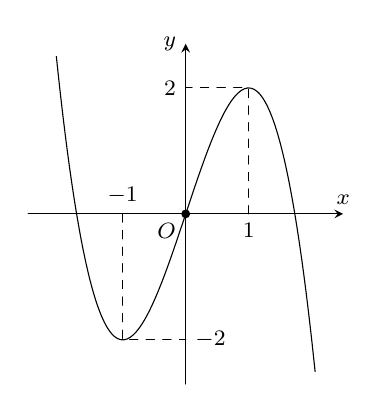
\begin{tikzpicture}[scale=0.8, font=\footnotesize,line join=round, line cap=round,>=stealth]
 			\draw[->] (-2.5,0)--(2.5,0) node[above]{$x$};
 			\draw[->] (0,-2.7)--(0,2.7) node[left]{$y$};
 			\draw[dashed] (1,0)|-(0,2);
 			\draw[dashed] (-1,0)|-(0,-2);
 			\begin{scope}
 				\clip (-2.5,2.5) rectangle (2.5,-2.5);
 				\draw plot[domain=-2.5:2.5,smooth,samples=100]
 				(\x,{-(\x)^3+3*(\x)});
 			\end{scope}
 			\fill (0,0) circle(2pt); 
 			\path 
 			(0,0) node[below left]{$O$}
 			(1,0) node[below]{$1$}
 			(-1,0) node[above]{$-1$}
 			(0,2) node[left]{$2$}
 			(0,-2) node[right]{$-2$}
 			;
 	\end{tikzpicture}}
 	\loigiai{
 	\immini{Đường thẳng $y=-1$ cắt đồ thị hàm số $y=f(x)$ tại ba điểm phân biệt, trong đó có hai điểm có hoành độ âm và một điểm có hoành độ dương.\\
 	Vậy phương trình $f(x)=-1$ có đúng một nghiệm thực dương.}
 	{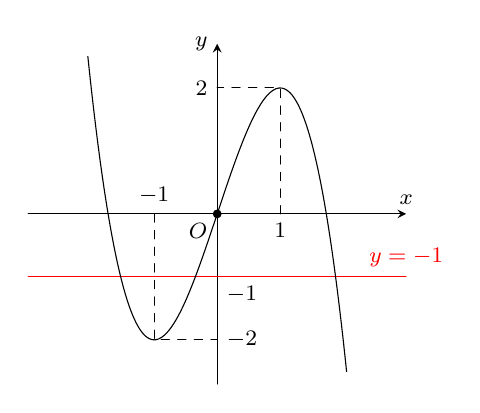
\begin{tikzpicture}[scale=0.8, font=\footnotesize,line join=round, line cap=round,>=stealth]
 			\draw[->] (-3,0)--(3,0) node[above]{$x$};
 			\draw[->] (0,-2.7)--(0,2.7) node[left]{$y$};
 			\draw[dashed] (1,0)|-(0,2);
 			\draw[dashed] (-1,0)|-(0,-2);
 			\draw[red] (-3,-1)--(3,-1)node[above]{$y=-1$};
 			\begin{scope}
 				\clip (-2.5,2.5) rectangle (2.5,-2.5);
 				\draw plot[domain=-2.5:2.5,smooth,samples=100]
 				(\x,{-(\x)^3+3*(\x)});
 			\end{scope}
 			\fill (0,0) circle(2pt); 
 			\path 
 			(0,0) node[below left]{$O$}
 			(1,0) node[below]{$1$}
 			(-1,0) node[above]{$-1$}
 			(0,2) node[left]{$2$}
 			(0,-2) node[right]{$-2$}
 			(0,-1) node[below right]{$-1$}
 			;
 	\end{tikzpicture}}	
 	}
\end{ex}


\begin{ex}%[2-GHK1, THPT Hiệp Đức - Quảng Nam, 2020 - 2021]%[Đỗ Đường Hiếu, 12-EX3-20]%[2D1B5-3]
	\immini{Cho hàm số $y=f(x)$ có đồ thị như hình vẽ. Tìm số nghiệm thực của phương trình $4f(x)+3=0$.
		\choice
		{\True $2$}
		{$3$}
		{$4$}
		{$0$}}
	{\begin{tikzpicture}[scale=0.8, font=\footnotesize,line join=round, line cap=round,>=stealth]
			\draw[->] (-2.5,0)--(2.5,0) node[above]{$x$};
			\draw[->] (0,-2.5)--(0,2) node[left]{$y$};
			\draw[dashed] (1,0)|-(0,1)-|(-1,0);
			\begin{scope}
				\clip (-2.5,2) rectangle (2.5,-2);
				\draw plot[domain=-2.5:4.5,smooth,samples=100]
				(\x,{-(\x)^4+2*(\x)^2});
			\end{scope}
			\fill (0,0) circle(2pt); 
			\path 
			(0,0) node[below left]{$O$}
			(1,0) node[below]{$1$}
			(-1,0) node[below]{$-1$}
			(0,1) node[above left]{$1$}
			;
	\end{tikzpicture}}
	\loigiai{
	Ta có $4f(x)+3=0\Leftrightarrow f(x)=-\dfrac{3}{4}$.\qquad $(*)$\\
	Đường thẳng $y=-\dfrac{3}{4}$ cắt đồ thị hàm số $y=f(x)$ tại $2$ điểm phân biệt. Do đó phương trình $(*)$ có $2$ nghiệm thực phân biệt.	
	}
\end{ex}


\begin{ex}%[2-GHK1, THPT Hiệp Đức - Quảng Nam, 2020 - 2021]%[Đỗ Đường Hiếu, 12-EX3-20]%[2D1K5-1]
	\immini{Cho hàm số bậc ba $y=ax^3+bx^2+cx+d$ ($a\ne 0$) có đồ thị như hình vẽ. Mệnh đề nào sau đây đúng?
		\choice
		{\True $a>0$, $b<0$, $c<0$, $d>0$}
		{$a>0$, $b>0$, $c>0$, $d>0$}
		{$a>0$, $c>0>b$, $d<0$}
		{$a>0$, $b>0$, $c>0$, $d>0$}}
	{\begin{tikzpicture}[scale=0.8, font=\footnotesize,line join=round, line cap=round,>=stealth]
			\draw[->] (-2.5,0)--(4.5,0) node[above]{$x$};
			\draw[->] (0,-2.5)--(0,3) node[left]{$y$};
			\draw[dashed] (-0.5,0)|-(0,85/48);
			\draw[dashed] (2,0)|-(0,-5/6);
			\begin{scope}
				\clip (-2.5,2.5) rectangle (4,-2);
				\draw plot[domain=-2.5:4,smooth,samples=100]
				(\x,{(1/3)*(\x)^3-0.75*(\x)^2-(\x)+1.5});
			\end{scope}
			\fill (0,0) circle(2pt); 
			\path 
			(0,0) node[below left]{$O$}
			;
	\end{tikzpicture}}
	\loigiai{
	Từ dáng điệu của đồ thị ta có $a>0$.\\
	Đồ thị cắt trục tung $Oy$ tại điểm $(0;d)$, do đó $d>0$.\\
	Ta có $y'=3ax^2+2bx+c$.\\
	Từ đồ thị hàm số ta suy ra $y'=0$ có hai nghiệm $x_1$, $x_2$ và
	\[\heva{&x_1x_2<0\\&x_1+x_2>0}\Leftrightarrow\heva{&\dfrac{c}{3a}<0\\&-\dfrac{2b}{3a}>0}\Leftrightarrow\heva{&\dfrac{c}{a}<0\\&\dfrac{b}{a}<0.}\]
	Do $a>0$ nên suy ra	$b<0$ và $c<0$.\\
	Như vậy $a>0$, $b<0$, $c<0$, $d>0$. 
	}
\end{ex}

\begin{ex}%[2-GHK1, THPT Hiệp Đức - Quảng Nam, 2020 - 2021]%[Đỗ Đường Hiếu, 12-EX3-20]%[2D1K5-3]
	\immini{Cho hàm số $y=f(x)$ liên tục trên $\mathbb{R}$ và có đồ thị như hình vẽ. Phương trình $f\left(f(x)-1\right)=0$ có tất cả bao nhiêu nghiệm thực phân biệt?
		\choice
		{\True $7$}
		{$6$}
		{$5$}
		{$9$}}
	{\begin{tikzpicture}[scale=0.8, font=\footnotesize,line join=round, line cap=round,>=stealth]
			\draw[->] (-3,0)--(3,0) node[above]{$x$};
			\draw[->] (0,-4.3)--(0,2.5) node[left]{$y$};
			\draw[dashed] (1,0)|-(0,-3)-|(-2,0);
			\draw[dashed] (-1,0)|-(0,1)-|(2,0);
			\begin{scope}
				\clip (-2.5,2) rectangle (2.5,-4);
				\draw plot[domain=-2.5:2.5,smooth,samples=100]
				(\x,{(\x)^3-3*(\x)-1});
			\end{scope}
			\fill (0,0) circle(2pt); 
			\path 
			(0,0) node[below right]{$O$}
			(1,0) node[above]{$1$}
			(-2,0) node[above]{$-2$}
			(-1,0) node[below]{$-1$}
			(2,0) node[below]{$2$}
			(0,1) node[above right]{$1$}
			(0,-3) node[below right]{$-3$}
			;
	\end{tikzpicture}}
	\loigiai{
	Từ đồ thị hàm số ta suy ra $f(t)=0\Leftrightarrow\hoac{&t=t_1\in (-2;-1)\\&t=t_2\in (-1;0)\\&t=t_3\in (1;2).}$\\
	Do đó $f\left(f(x)-1\right)=0\Leftrightarrow\hoac{&f(x)-1=t_1\in (-2;-1)\\&f(x)-1=t_2\in (-1;0)\\&f(x)-1=t_3\in (1;2)}\Leftrightarrow\hoac{&f(x)=t_1+1\in (-1;0)\\&f(x)=t_2+1\in (0;1)\\&f(x)=t_3+1\in (2;3).}$\\
	Dựa vào đồ thị hàm số $y=f(x)$ ta có
	\begin{itemize}
		\item Phương trình $f(x)=t_1+1\in (-1;0)$ có $3$ nghiệm phân biệt.
		\item Phương trình $f(x)=t_2+1\in (0;1)$ có $3$ nghiệm phân biệt.
		\item Phương trình $f(x)=t_3+1\in (2;3)$ có $1$ nghiệm.
	\end{itemize}
Dễ thấy rằng các nghiệm trên đôi một phân biệt. Do đó phương trình $f\left(f(x)-1\right)=0$ có $7$ nghiệm phân biệt.
	}
\end{ex}


\begin{ex}%[2-GHK1, THPT Hiệp Đức - Quảng Nam, 2020 - 2021]%[Đỗ Đường Hiếu, 12-EX3-20]%[2H1Y1-2]
	\immini{Khối đa diện trong hình vẽ bên có bao nhiêu mặt?
		\choice
		{\True $9$}
		{$7$}
		{$8$}
		{$10$}}
	{\begin{tikzpicture}[scale=1, font=\footnotesize,line join=round, line cap=round,>=stealth]
			\path 
			(0,0) coordinate (A)
			(2,1) coordinate (B)
			(A)+(4,0) coordinate (D)
			(B)+(4,0) coordinate (C)
			(A)+(0,2) coordinate (A1)
			(B)+(0,2) coordinate (B1)
			(D)+(0,2) coordinate (D1)
			(C)+(0,2) coordinate (C1)
			(A1)+(0.7,1) coordinate (A3)
			(B1)+(0.7,1) coordinate (B3)
			($(A3)!0.15!(B3)$) coordinate (A2)
			($(A3)!0.85!(B3)$) coordinate (B2)
			;
			\draw 
			(A)--(D)--(C)
			(A1)--(D1)--(C1)
			(A1)--(A2)--(D1)
			(A2)--(B2)--(C1)
			(A)--(A1) (D)--(D1)	(C)--(C1)		;
			\draw[dashed]
			(A)--(B)--(C)
			(A1)--(B1)--(C1)
			(B)--(B1)--(B2);
			
	\end{tikzpicture}}
	\loigiai{
	Khối đa diện đã cho có tất cả $9$ mặt.	
	}
\end{ex}

 
\begin{ex}%[2-GHK1, THPT Hiệp Đức - Quảng Nam, 2020 - 2021]%[Đỗ Đường Hiếu, 12-EX3-20]%[2H1Y1-3]
	Mặt phẳng $(AB'C')$ chia khối lăng trụ $ABC.A'B'C'$ thành các khối đa diện nào?
		\choice
		{\True Một khối chóp tam giác và một khối chóp tứ giác}
		{Một khối chóp tam giác và một khối chóp ngũ giác}
		{Hai khối chóp tứ giác}
		{Hai khối chóp tam giác}
	\loigiai{
	\immini{Mặt phẳng $(AB'C')$ chia khối lăng trụ $ABC.A'B'C'$ thành khối chóp tam giác $A.A'B'C'$ và khối chóp tứ giác $A.BCC'B'$.}
	{\begin{tikzpicture}[scale=1, font=\footnotesize,line join=round, line cap=round,>=stealth]
			\path 
			(0,0) coordinate (A)
			(3,0) coordinate (B)
			(1,-1) coordinate (C)
			(A)+(0,3) coordinate (A')
			(B)+(0,3) coordinate (B')
			(C)+(0,3) coordinate (C')
			;
			\draw 
			(A')--(B')--(C')--cycle
			(A)--(C)--(B)
			(A)--(A') (B)--(B')	(C)--(C')	(A)--(C');
			\draw[dashed]
			(A)--(B) (A)--(B');
			\foreach \x/\g in {A/-110,B/-70,C/-70,A'/110,B'/50,C'/90} \fill[black] (\x) circle (1pt)
			($(\x)+(\g:3mm)$) node{$\x$};
	\end{tikzpicture}}	
	}
\end{ex}


\begin{ex}%[2-GHK1, THPT Hiệp Đức - Quảng Nam, 2020 - 2021]%[Đỗ Đường Hiếu, 12-EX3-20]%[2H1B2-1]
	Tâm tất cả các mặt của một khối lập phương là các đỉnh của khối nào sau đây?
	\choice
	{\True Bát diện đều}
	{Tứ diện đều}
	{Lục giác đều}
	{Ngũ giác đều}
	\loigiai{
		\immini{Tâm tất cả các mặt của một khối lập phương là các đỉnh của khối bát diện đều.}
		{\begin{tikzpicture}[scale=1, font=\footnotesize,line join=round, line cap=round,>=stealth]
			\path 
			(0,0) coordinate (A)
			(2,1) coordinate (B)
			(A)+(5,0) coordinate (D)
			(B)+(5,0) coordinate (C)
			(A)+(0,4) coordinate (A1)
			(B)+(0,4) coordinate (B1)
			(D)+(0,4) coordinate (D1)
			(C)+(0,4) coordinate (C1)
			($(A)!0.5!(C)$) coordinate (M)
			($(A1)!0.5!(C1)$) coordinate (N)
			($(A)!0.5!(B1)$) coordinate (P)
			($(C)!0.5!(D1)$) coordinate (Q)
			($(A)!0.5!(D1)$) coordinate (E)
			($(B)!0.5!(C1)$) coordinate (F)
			;
			\draw 
			(A)--(D)--(C)
			(A1)--(D1)--(C1)
			(A)--(A1) (D)--(D1)	(C)--(C1)
			(A1)--(B1)--(C1) 
			;
			\draw[dashed]
			(A)--(B)--(C)
			(B)--(B1)
			(M)--(P) (M)--(Q) (M)--(E) (M)--(F)
			(N)--(P) (N)--(Q) (N)--(E) (N)--(F)
			(P)--(E)--(Q)--(F)--cycle
			;
			
	\end{tikzpicture}}	
	}
\end{ex}


\begin{ex}%[2-GHK1, THPT Hiệp Đức - Quảng Nam, 2020 - 2021]%[Đỗ Đường Hiếu, 12-EX3-20]%[2H1Y3-2]
	Cho khối chóp có diện tích đáy $S=3$ và chiều cao $h=4$. Tính thể tích của khối chóp đã cho.
	\choice
	{\True $4$}
	{$6$}
	{$12$}
	{$36$}
	\loigiai{
	Thể tích của khối chóp đã cho là $V=\dfrac{1}{3}Sh=\dfrac{1}{3}\cdot 3\cdot 4=4$.
	}
\end{ex}


\begin{ex}%[2-GHK1, THPT Hiệp Đức - Quảng Nam, 2020 - 2021]%[Đỗ Đường Hiếu, 12-EX3-20]%[2H1B3-2]
	Cho hình chóp tứ giác $S.ABCD$ có đáy $ABCD$ là hình vuông cạnh $a$, cạnh $SA$ vuông góc với mặt phẳng đáy và $SA=a\sqrt{2}$. Tính thể tích của khối chóp $S.ABCD$.
	\choice
	{\True $\dfrac{\sqrt{2}a^3}{3}$}
	{$\dfrac{\sqrt{2}a^3}{6}$}
	{$\sqrt{2}a^3$}
	{$\dfrac{\sqrt{2}a^3}{2}$}
	\loigiai{
	\immini{Thể tích khối chóp $S.ABCD$ là
	\[V=\dfrac{1}{3}S_{ABCD}\cdot SA=\dfrac{1}{3}\cdot a^2\cdot a\sqrt{2}=\dfrac{\sqrt{2}a^3}{3}.\]}
	{\begin{tikzpicture}[scale=1, font=\footnotesize,line join=round, line cap=round,>=stealth]
			\path 
			(0,0) coordinate (A)
			(-1,-1) coordinate (B)
			(B)+(3,0) coordinate (C)
			(A)+(3,0) coordinate (D)
			(A)+(0,3) coordinate (S)
			;
			\draw 
			(B)--(C)--(D)
			(S)--(B) (S)--(C) (S)--(D);
			\draw[dashed]
			(B)--(A)--(D) (S)--(A);
			\foreach \x/\g in {A/-110,B/-70,C/-70,D/-70,S/90} \fill[black] (\x) circle (1pt)
			($(\x)+(\g:3mm)$) node{$\x$};
			\tkzMarkRightAngles(S,A,B S,A,D)
	\end{tikzpicture}}		
	}
\end{ex}


\begin{ex}%[2-GHK1, THPT Hiệp Đức - Quảng Nam, 2020 - 2021]%[Đỗ Đường Hiếu, 12-EX3-20]%[2H1B3-4]
	Cho hình chóp $S.ABC$ có đáy là tam giác đều cạnh $a$, cạnh bên $SA$ vuông góc với đáy và thể tích của khối chóp đó bằng $\dfrac{a^3}{4}$. Tính độ dài cạnh bên $SA$.
	\choice
	{\True $a\sqrt{3}$}
	{$\dfrac{a\sqrt{3}}{3}$}
	{$\dfrac{a\sqrt{3}}{2}$}
	{$2a\sqrt{3}$}
	\loigiai{
	\immini{Diện tích tam giác $ABC$ là $S_{ABC}=\dfrac{a^2\sqrt{3}}{4}$. Do đó
		\[V=\dfrac{1}{3}S_{ABC}\cdot SA\Rightarrow SA=\dfrac{3V}{S_{ABC}}=\dfrac{3\cdot\dfrac{a^3}{4}}{\dfrac{a^2\sqrt{3}}{4}}=a\sqrt{3}.\]}
	{\begin{tikzpicture}[scale=1, font=\footnotesize,line join=round, line cap=round,>=stealth]
			\path 
			(0,0) coordinate (A)
			(2,-1) coordinate (B)
			(3,0) coordinate (C)
			(A)+(0,3) coordinate (S)
			;
			\draw 
			(A)--(B)--(C)
			(S)--(A) (S)--(B) (S)--(C);
			\draw[dashed]
			(C)--(A);
			\foreach \x/\g in {A/-110,B/-70,C/-70,S/90} \fill[black] (\x) circle (1pt)
			($(\x)+(\g:3mm)$) node{$\x$};
			\tkzMarkRightAngles(S,A,B S,A,C)
	\end{tikzpicture}}		
	}
\end{ex}


\begin{ex}%[2-GHK1, THPT Hiệp Đức - Quảng Nam, 2020 - 2021]%[Đỗ Đường Hiếu, 12-EX3-20]%[2H1B3-2]
	Cho khối lăng trụ đứng $ABC.A'B'C'$ có $B'C=3a$, đáy $ABC$ là tam giác vuông cân tại $B$ và $AC=a\sqrt{2}$. Tính thể tích $V$ của khối lăng trụ đứng $ABC.A'B'C'$.
	\choice
	{\True $V=\sqrt{2}a^3$}
	{$V=\dfrac{a^3}{6\sqrt{2}}$}
	{$V=\dfrac{\sqrt{2}a^3}{3}$}
	{$V=2a^3\sqrt{2}$}
	\loigiai{
	\immini{Do tam giác $ABC$ vuông cân tại $B$ và $AC=a\sqrt{2}$ nên suy ra $BA=BC=a$.\\
	Trong tam giác $B'BC$ vuông tại $B$, ta có
\[BB'=\sqrt{B'C^2-BC^2}=\sqrt{(3a)^2-a^2}=2a\sqrt{2}.\]
Thể tích $V$ của khối lăng trụ đứng $ABC.A'B'C'$ là
\[V=S_{BAC}\cdot BB'=\dfrac{1}{2}a^2\cdot 2a\sqrt{2}=\sqrt{2}a^3.\] }
	{\begin{tikzpicture}[scale=1, font=\footnotesize,line join=round, line cap=round,>=stealth]
			\path 
			(0,0) coordinate (A)
			(3,0) coordinate (B)
			(1,-1) coordinate (C)
			(A)+(0,3) coordinate (A')
			(B)+(0,3) coordinate (B')
			(C)+(0,3) coordinate (C')
			;
			\draw 
			(A')--(B')--(C')--cycle
			(A)--(C)--(B)
			(A)--(A') (B)--(B')	(C)--(C');
			\draw[dashed]
			(A)--(B);
			\foreach \x/\g in {A/-110,B/-70,C/-70,A'/110,B'/50,C'/90} \fill[black] (\x) circle (1pt)
			($(\x)+(\g:3mm)$) node{$\x$};
	\end{tikzpicture}}		
	}
\end{ex}


\begin{ex}%[2-GHK1, THPT Hiệp Đức - Quảng Nam, 2020 - 2021]%[Đỗ Đường Hiếu, 12-EX3-20]%[2H1B3-2]
	Cho khối chóp $S.ABC$ có đáy $ABC$ là tam giác vuông tại $B$, $AB=a$, $AC=2a$, $SA\perp (ABC)$ và $SA=a$. Tính thể tích của khối chóp $S.ABC$.
	\choice
	{\True $\dfrac{a^3\sqrt{3}}{6}$}
	{$\dfrac{a^3\sqrt{3}}{3}$}
	{$\dfrac{2a^3}{3}$}
	{$\dfrac{a^3\sqrt{3}}{2}$}
	\loigiai{
	\immini{
	Ta có $BC=\sqrt{AC^2-AB^2}=\sqrt{(2a)^2-a^2}=a\sqrt{3}$.\\
Diện tích tam giác $ABC$ là $S_{ABC}=\dfrac{1}{2}AB\cdot BC=\dfrac{1}{2}a\cdot a\sqrt{3}=\dfrac{a^2\sqrt{3}}{2}$.\\
Thể tích của khối chóp $S.ABC$ là
\[V=\dfrac{1}{3}S_{ABC}\cdot SA=\dfrac{1}{3}\cdot\dfrac{a^2\sqrt{3}}{2}\cdot a=\dfrac{a^3\sqrt{3}}{6}.\]}
	{\begin{tikzpicture}[scale=1, font=\footnotesize,line join=round, line cap=round,>=stealth]
			\path 
			(0,0) coordinate (A)
			(2,-1) coordinate (B)
			(3,0) coordinate (C)
			(A)+(0,3) coordinate (S)
			;
			\draw 
			(A)--(B)--(C)
			(S)--(A) (S)--(B) (S)--(C);
			\draw[dashed]
			(C)--(A);
			\foreach \x/\g in {A/-110,B/-70,C/-70,S/90} \fill[black] (\x) circle (1pt)
			($(\x)+(\g:3mm)$) node{$\x$};
			\tkzMarkRightAngles(S,A,B S,A,C A,B,C)
	\end{tikzpicture}}		
	}
\end{ex}


\begin{ex}%[2-GHK1, THPT Hiệp Đức - Quảng Nam, 2020 - 2021]%[Đỗ Đường Hiếu, 12-EX3-20]%[2H1K3-2]
	Cho khối chóp $S.ABCD$ có đáy là hình vuông cạnh $a\sqrt{2}$, tam giác $SAC$ vuông tại $S$ và nằm trong mặt phẳng vuông góc với đáy, cạnh bên $SA$ tạo với đáy góc $60^\circ$. Tính thể tích $V$ của khối chóp $S.ABD$.
	\choice
	{\True $V=\dfrac{a^3\sqrt{3}}{6}$}
	{$V=\dfrac{a^3\sqrt{3}}{12}$}
	{$V=a^3\sqrt{3}$}
	{$V=\dfrac{a^3\sqrt{3}}{3}$}
	\loigiai{
	\immini{
		Tam giác $SAC$ vuông tại $S$ và nằm trong mặt phẳng vuông góc với đáy $(ABCD)$ nên suy ra $AC$ là hình chiếu vuông góc của $AS$ trên mặt phẳng $(ABCD)$. Do đó 
	\[\widehat{\left(SA;(ABCD)\right)}=\widehat{\left(SA;AC\right)}=\widehat{SAC}\Rightarrow \widehat{SAC}=60^\circ.\]
	Kẻ $SH\perp AC$ tại $H$, suy ra $SH\perp (ABCD)$.\\
Hình vuông $ABCD$ có cạnh $a\sqrt{2}$ nên suy ra 
$$AC=a\sqrt{2}\cdot \sqrt{2}=2a.$$
Ta có $SA=AC\cdot \cos\widehat{SAC}=2a\cdot \cos 60^\circ =a$.\\
Từ đó $SH=SA\cdot \sin\widehat{SAC}=a\cdot\sin 60^\circ =\dfrac{a\sqrt{3}}{2}$.\\
Thể tích khối chóp $S.ABD$ là
\[V=\dfrac{1}{3}\cdot S_{ABD}\cdot SH=\dfrac{1}{3}\cdot\dfrac{1}{2}\cdot (a\sqrt{2})^2\cdot \dfrac{a\sqrt{3}}{2}=\dfrac{a^3\sqrt{3}}{6}.\] }
	{\begin{tikzpicture}[scale=1, font=\footnotesize,line join=round, line cap=round,>=stealth]
			\path 
			(0,0) coordinate (A)
			(-1.5,-1.5) coordinate (B)
			(A)+(4,0) coordinate (D)
			(B)+(4,0) coordinate (C)
			(1,3) coordinate (S)
			($(A)!0.6!(C)$) coordinate (H)
			;
			\draw 
			(B)--(C)--(D)
			(S)--(D) (S)--(B) (S)--(C);
			\draw[dashed]
			(B)--(A)--(D)  (S)--(A) (A)--(C)
			(S)--(H);
			\foreach \x/\g in {A/-110,B/-70,C/-70,D/-60,H/-90,S/90} \fill[black] (\x) circle (1pt)
			($(\x)+(\g:3mm)$) node{$\x$};
			\tkzMarkRightAngles(A,S,C S,H,A)
	\end{tikzpicture}}		
	}
\end{ex}


\begin{ex}%[2-GHK1, THPT Hiệp Đức - Quảng Nam, 2020 - 2021]%[Đỗ Đường Hiếu, 12-EX3-20]%[2H1K3-2]
	Cho lăng trụ đều $ABC.A'B'C'$. Biết rằng góc giữa $(A'BC)$ và $(ABC)$ là $30^\circ$, tam giác $A'BC$ có diện tích bằng $8$. Tính thể tích của khối lăng trụ $ABC.A'B'C'$.
	\choice
	{\True $8\sqrt{3}$}
	{$3\sqrt{3}$}
	{$24\sqrt{3}$}
	{$\dfrac{8\sqrt{3}}{3}$}
	\loigiai{
	\immini{Gọi $M$ là trung điểm $BC$, ta có $BC\perp (A'AM)$. Do đó góc giữa hai mặt phẳng $(A'BC)$ và $(ABC)$ bằng góc $\widehat{A'MA}\Rightarrow \widehat{A'MA}=30^\circ$.\\
	Đặt $AB=x$, ta có $AM=\dfrac{x\sqrt{3}}{2}$.\\
Ta có $A'M=\dfrac{AM}{\cos \widehat{A'MA}}=x$.\\
Diện tích tam giác $A'BC$ là
\[S_{A'BC}=\dfrac{1}{2}\cdot BC\cdot A'M=\dfrac{1}{2}\cdot x\cdot x=\dfrac{1}{2}x^2.\]
Do đó $S_{A'BC}=8\Leftrightarrow\dfrac{1}{2}x^2=8\Rightarrow x=4$.\\
Ta có $AA'=AM\cdot \tan\widehat{A'MA}=\dfrac{4\sqrt{3}}{2}\cdot \tan 30^\circ =2$.\\
Thể tích của khối lăng trụ $ABC.A'B'C'$ là
\[V=S_{ABC}\cdot AA'=\dfrac{4^2\sqrt{3}}{4}\cdot 2=8\sqrt{3}.\]}
	{\begin{tikzpicture}[scale=1, font=\footnotesize,line join=round, line cap=round,>=stealth]
			\path 
			(0,0) coordinate (A)
			(3,0) coordinate (B)
			(1,-1) coordinate (C)
			(A)+(0,3) coordinate (A')
			(B)+(0,3) coordinate (B')
			(C)+(0,3) coordinate (C')
			($(B)!0.5!(C)$) coordinate (M)
			;
			\draw 
			(A')--(B')--(C')--cycle
			(A)--(C)--(B)
			(A)--(A') (B)--(B')	(C)--(C') (A')--(C);
			\draw[dashed]
			(A)--(B) (A)--(M)--(A') (A')--(B);
			\foreach \x/\g in {A/-110,B/-70,C/-70,A'/110,B'/50,C'/90,M/-70} \fill[black] (\x) circle (1pt)
			($(\x)+(\g:3mm)$) node{$\x$};
	\end{tikzpicture}}		
	}
\end{ex}


\begin{ex}%[2-GHK1, THPT Hiệp Đức - Quảng Nam, 2020 - 2021]%[Đỗ Đường Hiếu, 12-EX3-20]%[2H1G3-2]
	Cho hình chóp $S.ABC$ có đáy là tam giác $ABC$ vuông tại $C$, $AB=2a$, $AC=a$ và $SA$ vuông góc với mặt phẳng $(ABC)$. Biết góc giữa hai mặt phẳng $(SAB)$ và $(SBC)$ bằng $60^\circ$. Tính thể tích của khối chóp $S.ABC$.
	\choice
	{\True $\dfrac{a^3\sqrt{6}}{12}$}
	{$\dfrac{a^3\sqrt{2}}{6}$}
	{$\dfrac{a^3\sqrt{6}}{4}$}
	{$\dfrac{a^3\sqrt{2}}{2}$}
	\loigiai{
	\immini{
		Ta có $BC=\sqrt{AB^2-AC^2}=\sqrt{(2a)^2-a^2}=a\sqrt{3}$.\\
		Kẻ $AK\perp SC$ tại $K$, suy ra $AK\perp (SBC)\Rightarrow AK\perp SB$.\qquad $(1)$\\
	Kẻ $AH\perp SB$ tại $H$.\qquad $(2)$\\
Từ $(1)$ và $(2)$ ta có $SB\perp (AHK)$. Suy ra góc giữa hai mặt phẳng $(SAB)$ và $(SBC)$ bằng góc giữa $HK$ và $AH$, bằng góc $\widehat{AHK}\Rightarrow \widehat{AHK}=60^\circ$.\\ 
Đặt $x=SA$, ta có $AH=\dfrac{SA\cdot AB}{\sqrt{SA^2+AB^2}}=\dfrac{2ax}{\sqrt{x^2+4a^2}}$.\\
Ta cũng có $AK=\dfrac{SA\cdot AC}{\sqrt{SA^2+AC^2}}=\dfrac{ax}{\sqrt{x^2+a^2}}$.\\
}
	{\begin{tikzpicture}[scale=1, font=\footnotesize,line join=round, line cap=round,>=stealth]
			\path 
			(0,0) coordinate (A)
			(2,-1) coordinate (C)
			(3,0) coordinate (B)
			(A)+(0,3) coordinate (S)
			($(S)!0.7!(C)$) coordinate (K)
			($(S)!0.4!(B)$) coordinate (H)
			;
			\draw 
			(A)--(C)--(B)
			(S)--(A) (S)--(B) (S)--(C) (A)--(K)--(H);
			\draw[dashed]
			(B)--(A) (A)--(H);
			\foreach \x/\g in {A/-110,B/-70,C/-70,K/0,H/30,S/90} \fill[black] (\x) circle (1pt)
			($(\x)+(\g:3mm)$) node{$\x$};
			\tkzMarkRightAngles(S,A,B S,A,C A,C,B A,K,H)
	\end{tikzpicture}}	
\noindent
Trong tam giác $AHK$ vuông tại $K$, ta có
\[AK=AH\cdot \sin \widehat{AHK}\Leftrightarrow \dfrac{ax}{\sqrt{x^2+a^2}}= \dfrac{2ax}{\sqrt{x^2+4a^2}}\cdot\sin 60^\circ\Rightarrow x=\dfrac{a\sqrt{2}}{2}.\]
Như vậy $SA=\dfrac{a\sqrt{2}}{2}$.\\
Thể tích của khối chóp $S.ABC$ là
\[V=\dfrac{1}{3}S_{ABC}\cdot SA=\dfrac{1}{3}\cdot \dfrac{1}{2}\cdot AC\cdot BC\cdot SA=\dfrac{1}{6}\cdot a\cdot a\sqrt{3}\cdot \dfrac{a\sqrt{2}}{2}=\dfrac{a^3\sqrt{6}}{12}.\] 	
	}
\end{ex}
\Closesolutionfile{ans}
\begin{indapan}{10}
	{ans/ans-2-GHK1-28-HiepDuc-QuangNam-21}
\end{indapan}